\begin{figure}[t]
\begin{center}
    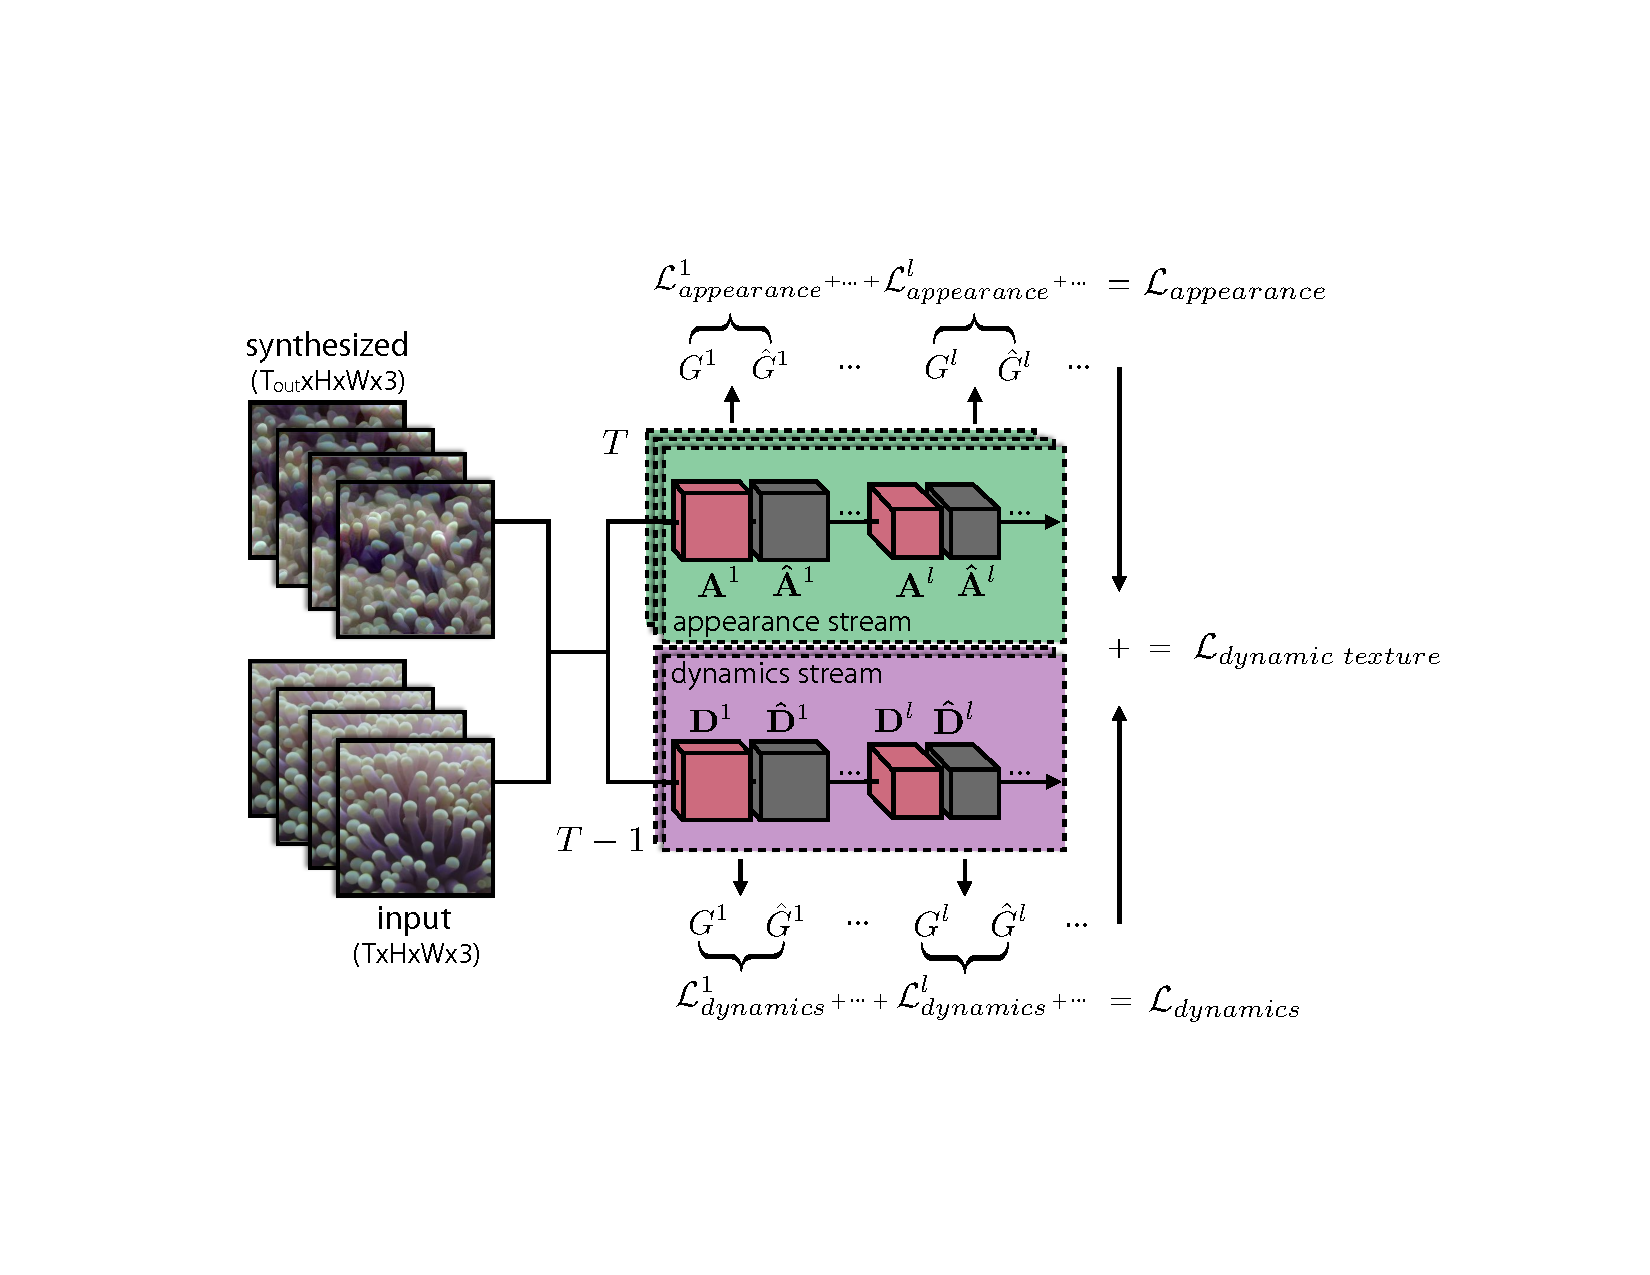
\epsfig{file=overallarchitecture.pdf, width = \textwidth}
\end{center}
\vspace{-0.45cm}
\caption[Two-stream dynamic texture generation.]{Two-stream dynamic texture generation.
Two sets of Gram matrices represent a dynamic texture's appearance and 
dynamics.
Matching these statistics allows for the generation of novel
textures as well as style transfer between textures. Here, $G^l$ and $\hat{G}^l$ are the Gram matrices of activations $A^l$ and $\hat{A}^l$ (or $D^l$ and $\hat{D}^l$) corresponding to the target and synthesized sequence, respectively, computed at layer $l$ of the appearance stream (or dynamics stream) and averaged over time $T$ (or $T-1$). $\mathcal{L}_\text{appearance}^l$ is the appearance loss at layer $l$, computed as the squared Frobenius norm between $G^l$ and $\hat{G}^l$ from the appearance stream. Similarly, $\mathcal{L}_\text{dynamics}^l$ is the dynamics loss at layer $l$ for the dynamics stream. By summing each loss computed at various layers, we arrive at $\mathcal{L}_\text{appearance}$ and $\mathcal{L}_\text{dynamics}$, which, when summed, form the combined dynamic texture loss, $\mathcal{L}_\text{dynamic texture}$, that is to be minimized.}
\label{fig:architecture}
\end{figure}
